
\documentclass[aspectratio=169]{beamer}
\usetheme{Boadilla}

\usepackage{qrcode}

\usepackage[utf8]{inputenc}       % Codificação de entrada
\usepackage[T1]{fontenc}          % Codificação de saída
\usepackage[portuguese]{babel}   % Idioma
\usepackage{XCharter}             % Fonte principal
\AtBeginDocument{\fontsize{12}{12}\selectfont}

%\usepackage{geometry}
%\geometry{papersize={210mm,150mm}}
\usepackage{tikz}
\usepackage{pgf-pie} % necessário para gráficos de pizza

\usepackage{color}
\usepackage{graphicx}
\usepackage{amsmath, amssymb, amsfonts}
\usepackage{bm}
\usepackage{booktabs}
\usepackage{multirow}
\usepackage{caption}
\usepackage{subfigure}
\usepackage{wrapfig}
\usepackage{multicol}
\usepackage{sidecap}
\usepackage{tikz}
\usepackage{listings}
\usepackage{siunitx}
\usepackage{pdfpages}
\usepackage{float}
\usepackage{hyperref}
\usepackage{academicons}
\usepackage{setspace}

\newcommand{\eng}[1]{\textsl{#1}}
\newcommand{\cod}[1]{\texttt{#1}}

\usepackage{tikz}
\usetikzlibrary{shapes.geometric, arrows, positioning}

% Definição de estilos para o fluxograma
\tikzstyle{startstop} = [ellipse, rounded corners, minimum width=2cm, minimum height=0.8cm, text centered, draw=black, fill=gray!20]
\tikzstyle{process} = [rectangle, minimum width=3.5cm, minimum height=1cm, text width=4.5cm, text centered, draw=black, fill=white]
\tikzstyle{decision} = [diamond, aspect=2, minimum width=3cm, minimum height=1cm, text centered, draw=black, fill=white]
\tikzstyle{arrow} = [thick,->,>=stealth]

% Definição de cores profissionais
\definecolor{mipsblue}{RGB}{50, 90, 120}
\definecolor{mipsred}{RGB}{150, 30, 30}

\title[Arquitetura de Computadores]{\huge  Redes neurais artificiais} %note that the optional arg in '[]' are displayed in the left column throughout the complete presentation
% adapt accordingly
% e.g., M.Sc. Intermediate Thesis Report
% or     B.Sc. Intermediate Thesis Report


\author[Prof. Dr. Oscar Eduardo Anacona Mosquera]{Prof. Dr. Oscar Eduardo Anacona Mosquera \newline\newline 
	\scriptsize{oscar.mosquera@ufmt.br}
}%note that the optional arg in '[]' are displayed in the left column throughout the complete presentation



\AtBeginSection[]
{
	\begin{frame}{Sumário}
		\tableofcontents[currentsection]
	\end{frame}
}


\begin{document}

	\begin{frame}[plain]
		\titlepage
	\end{frame}
	
	\begin{frame}{Sumário}
		\tableofcontents
	\end{frame}
	
%=======================================================================================
%\section{Introdução}
%=======================================================================================


\section{Introdução}




\begin{frame}{Rede neural}
	\justifying
	
	Um neurônio é a unidade básica do cérebro humano.
	
	
	
%	\begin{itemize}
%		\justifying
%		\item Somente a funcionalidade do circuito, não a estrutura.
%		
%		\item A descrição do hardware não está vinculada a uma implementação específica de hardware.
%		
%		
%		
%	\end{itemize}
	
	
	\begin{figure}[h]
		\centering
		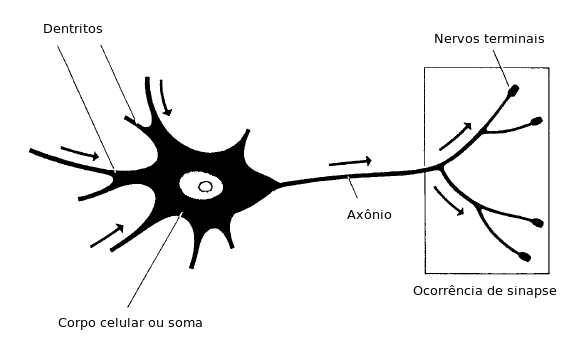
\includegraphics[width=0.67\textwidth]{Figs/fig01.png}
		
		{\small Fonte: Gonçalves}
	\end{figure}
	
	
\end{frame}



\begin{frame}{Rede Neural: modelo}
	\justifying
	
	Modelo de neurônio artificial proposto por McCulloch e Pitts. A soma é representada por uma composição de dois módulos: o primeiro é uma junção aditiva, somatório dos estímulos (sinais de entrada) multiplicado pelo seu fator excitatório (pesos sinápticos), e posteriormente uma função de ativação, que definirá, com base nas entradas e pesos sinápticos, qual será a saída do neurônio. O axônio é aqui representado pela saída ($y_k$) obtida pela aplicação da função de ativação.
	
	\begin{figure}[h]
		\centering
		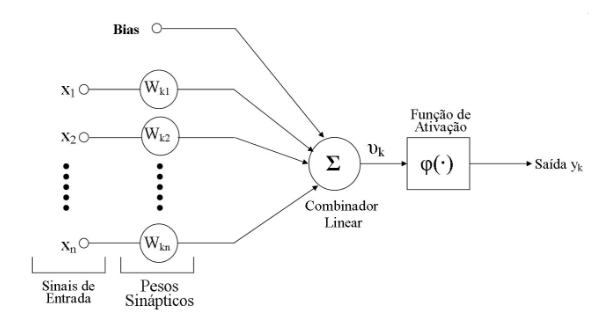
\includegraphics[width=0.5\textwidth]{Figs/fig02.png}
		%\caption{Modelo de McCulloch e Pitts.} % Opcional: adiciona uma legenda
		{\small Fonte: Gonçalves}
	\end{figure}
\end{frame}




\begin{frame}{Rede Neural: funções de ativação}
	\justifying
	
	
	\begin{figure}[h]
		\centering
		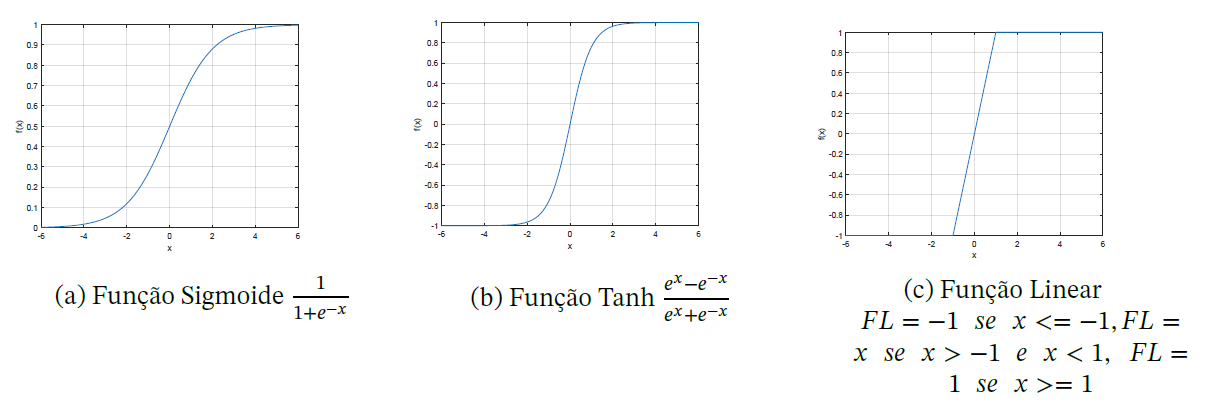
\includegraphics[width=0.9\textwidth]{Figs/fig03.png}
		{\small Fonte: TRIANA (2022)}
	%	\caption{Modelo de McCulloch e Pitts.} % Opcional: adiciona uma legenda
	\end{figure}
\end{frame}




\begin{frame}{Redes Multilayer Perceptron (MLP)}
	\justifying
	
	As redes MLP são redes do tipo \textit{feedforward} (alimentadas adiante) que possuem uma ou mais camadas de neurônios entre as camadas de entrada e saída, denominadas camadas ocultas.
	
	\begin{figure}[h]
		\centering
		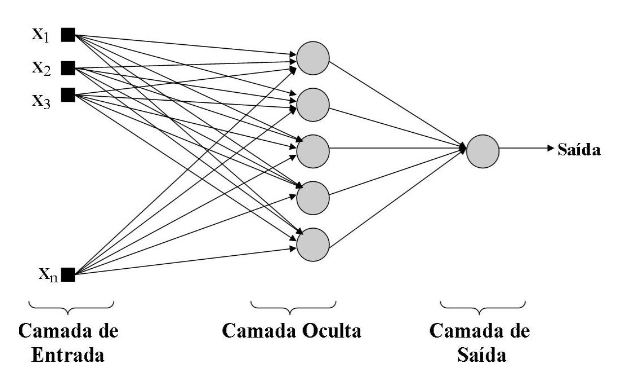
\includegraphics[width=0.6\textwidth]{Figs/fig04.png}
		%\caption{Arquitetura de uma rede Multilayer Perceptron.}
		{\small Fonte: Gonçalves}
	\end{figure}
	
	O algoritmo \textit{backpropagation} utiliza a técnica de busca por gradiente para minimizar a função de custo.
\end{frame}


\begin{frame}{Redes Multilayer Perceptron (MLP)}
	\justifying
	
	\begin{figure}[h]
		\centering
		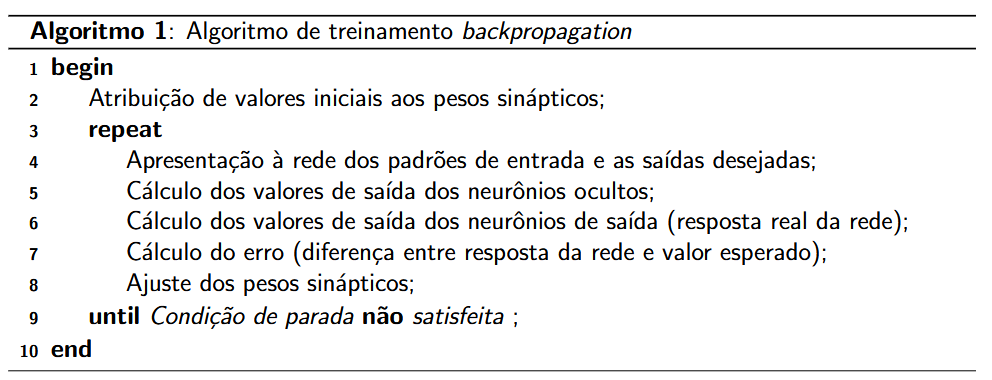
\includegraphics[width=0.8\textwidth]{Figs/fig05.png}
	%	\caption{Representação do processo de ajuste de pesos/otimização.}
	{\small Fonte: Gonçalves}
	\end{figure}
	
	% Se houver texto explicativo para esta imagem, ele pode ser inserido aqui.
\end{frame}


\begin{frame}{Redes Multilayer Perceptron (MLP)}
	\justifying
	
	Algumas soluções para contornar limitações do gradiente (como a convergência para mínimos locais) foram sugeridas, como a aplicação de outras técnicas de aprendizado de máquina conhecidas pela alta aplicabilidade em problemas de otimização global, tais como:
	
	\begin{itemize}
		\item Algoritmos Genéticos;
		\item Otimização por Colônia de Formigas (\textit{Ant Colony Optimization}).
		\item Otimização por enxame de partículas (PSO).
		\item Artifitial Bee Colony (ABC).
	\end{itemize}
\end{frame}






\begin{frame}{Como a Rede Aprende? (Backpropagation)}
	O algoritmo de \textbf{Retropropagação} é o método usado para treinar a rede neural. Ele funciona em um ciclo de "tentativa e erro":
	
	\begin{enumerate}
		\item \textbf{Passo à Frente (Forward):} A rede recebe os dados, faz os cálculos com os pesos atuais e gera um resultado.
		\item \textbf{Cálculo do Erro:} O computador compara o resultado da rede com a resposta correta e vê o tamanho do "vacilo" (erro).
		\item \textbf{Retropropagação (Backward):} O erro volta do final para o começo da rede, ajustando os \textbf{pesos} de cada neurônio.
		\item \textbf{Ajuste Fino:} O objetivo é diminuir o erro a cada rodada (época) até que a rede acerte quase tudo.
	\end{enumerate}
	
	\begin{block}{Por que treinar no Python?}
		Treinar exige muito cálculo matemático pesado. Fazemos o treinamento no PC (Python) e passamos apenas os \textbf{pesos prontos} para o FPGA.
	\end{block}
\end{frame}



% --- SLIDE 1: Classificação e Agrupamento ---
\begin{frame}{Aplicações das Redes Neurais }
	\justifying
	
	\begin{description}
		\item[Classificação de Padrões:] Consiste em classificar padrões de entrada em classes previamente conhecidas, tomando como base de conhecimento as características intrínsecas do problema.
		
		\vspace{0.5cm}
		
		\item[Clusterização:] Pode ser vista como um problema de classificação de padrões onde não se conhece previamente a quantidade ou a natureza das classes. A rede agrupa os dados por similaridade.
	\end{description}
\end{frame}

% --- SLIDE 2: Funções e Previsão ---
\begin{frame}{Aplicações das Redes Neurais }
	\justifying
	
	\begin{description}
		\item[Aproximação de Funções:] Utilizada para modelar funções complexas e de alta não linearidade. Quando algoritmos exatos falham, as redes neurais surgem como uma alternativa robusta para aproximação.
		
		\vspace{0.5cm}
		
		\item[Previsão:] Com base em um histórico de cenários e nas ações tomadas anteriormente, a rede é capaz de prever qual será a resposta ou o valor esperado em um novo cenário futuro.
	\end{description}
\end{frame}

% --- SLIDE 3: Otimização, Associação e Controle ---
\begin{frame}{Aplicações das Redes Neurais }
	\justifying
	
	\begin{description}
		\item[Otimização:] Consiste em encontrar o valor máximo ou mínimo de uma função objetivo, sendo muito utilizada em problemas de logística e engenharia.
		
		\vspace{0.3cm}
		
		\item[Associação:] Desenvolvimento de redes que associam padrões. Pode ser treinada com dados ruidosos (\textit{noise}) para identificar e recuperar o padrão original sem ruído.
		
		\vspace{0.3cm}
		
		\item[Controle:] Aplicação de redes neurais para auxiliar sistemas de controle adaptativo, ajustando parâmetros em tempo real para manter a estabilidade de um processo.
	\end{description}
\end{frame}




% --- SLIDE DE TRANSIÇÃO: O que é RBF? ---
\begin{frame}{Redes de Função de Base Radial (RBF)}
	\justifying
	Dentre as arquiteturas utilizadas para as aplicações citadas, as redes \textbf{RBF} se destacam pela sua simplicidade estrutural e rapidez de treinamento. 
	
	\begin{itemize}
		\item \textbf{Conceito:} Diferente das MLPs que utilizam funções sigmoides globais, as RBFs utilizam funções de ativação locais (geralmente Gaussianas).
		\item \textbf{Estrutura:} Composta por apenas três camadas:
		\begin{enumerate}
			\item \textbf{Entrada:} Apenas distribui os dados.
			\item \textbf{Oculta (Radial):} Calcula a distância entre a entrada e um centro pré-definido.
			\item \textbf{Saída (Linear):} Realiza uma combinação linear dos resultados.
		\end{enumerate}
	\end{itemize}
\end{frame}

% --- SLIDE DE MOTIVAÇÃO: Por que Hardware? ---
\begin{frame}{Motivação para Implementação em Hardware}
	\justifying
	Para aplicações de tempo real (como controle de sistemas industriais ou processamento de sinais de alta velocidade), a implementação em software nem sempre é eficiente.
	
	\begin{block}{Vantagens do Hardware Dedicado (FPGA/ASIC)}
		\begin{itemize}
			\item \textbf{Paralelismo:} Diferente de um processador comum que executa instruções em série, o hardware pode calcular todos os neurônios simultaneamente.
			\item \textbf{Baixa Latência:} Resposta quase instantânea aos estímulos de entrada.
			\item \textbf{Eficiência Energética:} Circuitos otimizados para uma única tarefa.
		\end{itemize}
	\end{block}
	
	A seguir, veremos como essa estrutura matemática é mapeada em blocos digitais.
\end{frame}













% --- SLIDE 1: Visão Geral e Neurônios ---
\begin{frame}{Arquitetura de Hardware RBF: Blocos Funcionais}
	\justifying
	A implementação digital da rede RBF é projetada para equilibrar paralelismo e consumo de área em hardware (FPGA/ASIC):
	
	\begin{columns}
		\begin{column}{0.5\textwidth}
			\textbf{Camada de Processamento:}
			\begin{itemize}
				\item \textbf{Blocos $N_1$ a $N_5$:} Instâncias dos neurônios da camada oculta.
				\item Calculam a função de base radial de forma paralela.
				\item Entradas ($r$) e centros ($c$) são roteados simultaneamente para os blocos.
			\end{itemize}
		\end{column}
		
		\begin{column}{0.5\textwidth}
			\begin{figure}
				\centering
				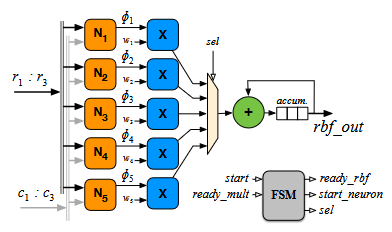
\includegraphics[width=\textwidth]{Figs/fig06.png}
				{\small Fonte: Sampaio (2018)}
			\end{figure}
		\end{column}
	\end{columns}
\end{frame}

% --- SLIDE 2: Datapath (Multiplicação e Acúmulo) ---
\begin{frame}{Arquitetura de Hardware RBF: Fluxo de Dados}
	\justifying
	Para converter as saídas dos neurônios no resultado final ($rbf\_out$), utiliza-se uma estrutura de \textbf{Multiplexação e Acúmulo}:
	
	\begin{itemize}
		\item \textbf{Multiplicadores ($X$):} Cada saída $\phi_i$ é ponderada pelo seu peso $w_i$ correspondente.
		\item \textbf{Multiplexador (MUX):} Seleciona sequencialmente cada produto para entrar no somador.
		\item \textbf{Somador/Acumulador:} Em vez de uma árvore de somadores (que gasta muita área), utiliza-se um registrador de acúmulo (\textit{accum}) para somar os termos um a um.
	\end{itemize}
\end{frame}






% --- SLIDE 4: Otimização de Kernel (Gaussiano vs Polinomial) ---
\begin{frame}{Otimização de Hardware: Kernels}
	\justifying
	Um dos maiores desafios em hardware é a implementação da função Gaussiana devido à exponencial ($\exp$). Uma alternativa comum é o uso de \textbf{aproximações polinomiais}:
	
	\begin{itemize}
		\item \textbf{Kernel Gaussiano:} Alta precisão biológica/matemática, porém exige mais recursos (Elementos Lógicos) para implementar a exponencial.
		\item \textbf{Kernel Polinomial:} Exige significativamente menos hardware, sendo implementado apenas com multiplicadores e somadores simples.
	\end{itemize}
	
	\begin{figure}
		\centering
		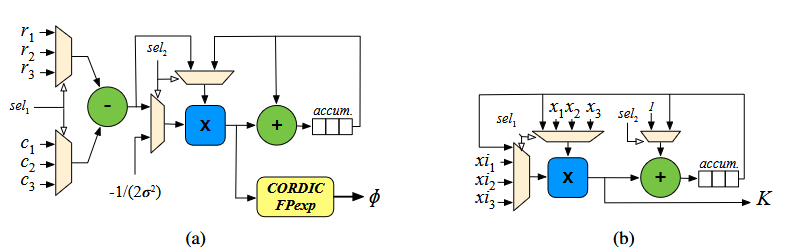
\includegraphics[width=0.7\textwidth]{Figs/fig07.png}
		{\small Fonte: Sampaio (2018)}
	\end{figure}
\end{frame}






% --- SLIDE 1: O caso simples (AND/OR) ---
\begin{frame}{Classificação de Padrões: Problemas Lineares}
	\justifying
	
	Muitas operações lógicas, como as portas \textbf{AND} e \textbf{OR}, são classificadas como problemas \textbf{linearmente separáveis}. Nesses casos, uma única reta (hiperplano) é capaz de dividir as classes no espaço de estados.
	
	\begin{figure}
		\centering
		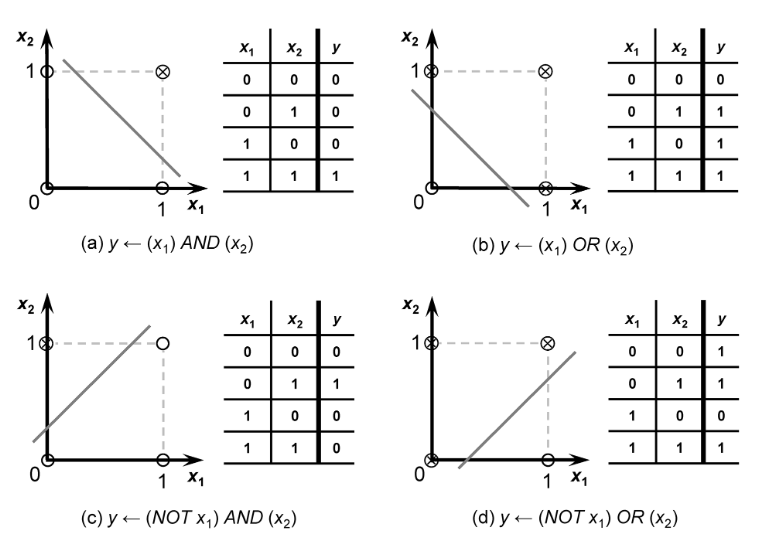
\includegraphics[width=0.45\textwidth]{Figs/fig10.png}
		\caption*{Exemplos de operações lógicas linearmente separáveis.}
		{\footnotesize Fonte: Silva, Spatti e Flauzino (2010).}
	\end{figure}
\end{frame}

% --- SLIDE 2: O Modelo (Neurônio Simples) ---
\begin{frame}{Classificação de Padrões: Modelo de Neurônio}
	\justifying
	
	Para resolver problemas lineares, utiliza-se a arquitetura de um neurônio artificial simples (Perceptron), composto por duas entradas ($x_1, x_2$) e uma saída ($y$).
	
	\begin{figure}
		\centering
		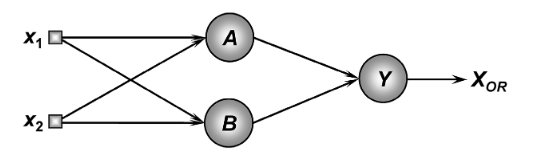
\includegraphics[width=0.55\textwidth]{Figs/fig09.png}
		\caption*{Representação de um neurônio com duas entradas e uma saída.}
		{\footnotesize Fonte: Silva, Spatti e Flauzino (2010).}
	\end{figure}
\end{frame}

% --- SLIDE 3: O Problema do XOR ---
\begin{frame}{Classificação de Padrões: Problemas Não Lineares}
	\justifying
	
	Na operação \textbf{ou-exclusivo (XOR)}, constata-se que seria impossível posicionar uma única reta que permitisse separar as duas classes resultantes. Este é um exemplo clássico de um problema \textbf{não linearmente separável}.
	
	\begin{figure}
		\centering
		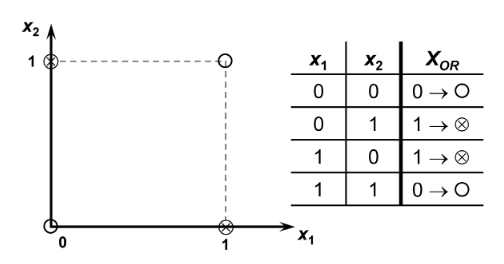
\includegraphics[width=0.6\textwidth]{Figs/fig08.png}
		\caption*{Distribuição espacial das classes da porta XOR.}
		{\footnotesize Fonte: Silva, Spatti e Flauzino (2010).}
	\end{figure}
\end{frame}

% --- SLIDE 4: Regiões Disjuntas ---
\begin{frame}{Classificação de Padrões: Regiões Disjuntas}
	\justifying
	
	Para solucionar problemas de maior complexidade e com regiões disjuntas, é necessário o uso de múltiplas camadas ou funções de base radial, permitindo criar fronteiras de decisão complexas.
	
	\begin{figure}
		\centering
		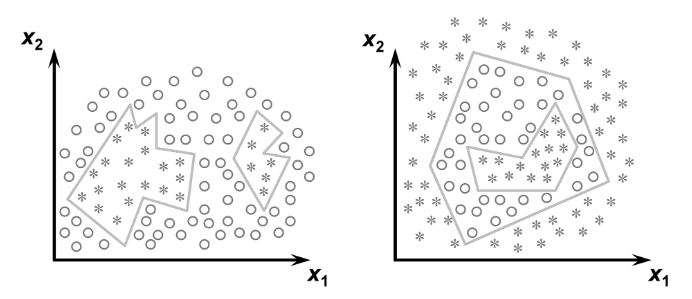
\includegraphics[width=0.7\textwidth]{Figs/fig11.png}
		\caption*{Exemplos de regiões disjuntas em classificação de padrões.}
		{\footnotesize Fonte: Silva, Spatti e Flauzino (2010).}
	\end{figure}
\end{frame}








\section{Ponto Flutuante}

% --- SLIDE: Representação Numérica ---
\begin{frame}{Representação Numérica: Ponto Flutuante (IEEE-754)}
	\justifying
	Para garantir a precisão dos cálculos neurais, utilizou-se o padrão \textbf{IEEE-754} de 32 bits. Contudo, em hardware, há um compromisso direto entre precisão e consumo de recursos.
	
	\begin{itemize}
		\item \textbf{Sinal (1 bit):} Define se o número é positivo ou negativo.
		\item \textbf{Expoente (8 bits):} Define a magnitude do número.
		\item \textbf{Mantissa (23 bits):} Define a precisão decimal.
	\end{itemize}
	
	\begin{block}{Otimização de Recursos}
		Em FPGAs, multiplicadores de ponto flutuante consomem muitos \textit{DSP Blocks}. Uma técnica explorada foi a \textbf{redução da mantissa} para observar a economia de elementos lógicos frente ao erro de aproximação.
	\end{block}
\end{frame}



% --- SLIDE: Exemplo de Conversão IEEE-754 ---
\begin{frame}{Conversão Manual: Exemplo com o número 6,5}
	\justifying
	Para representar o número $6,5_{10}$ no padrão IEEE-754 de 32 bits:
	
	\begin{enumerate}
		\item \textbf{Binário:} $6_{10} = 110$ e $0,5_{10} = 0,1 \implies \mathbf{110,1_2}$
		\item \textbf{Normalização:} $1,101 \times 2^2$ (movemos a vírgula 2 casas).
		\item \textbf{Sinal ($S$):} $0$ (positivo).
		\item \textbf{Expoente ($E$):} $E = \text{deslocamento} + 127 = 2 + 127 = 129_{10}$ \\
		Em binário: $\mathbf{10000001_2}$
		\item \textbf{Mantissa ($M$):} Parte fracionária de $1,101$ (omitindo o "1," implícito). \\
		Resultado (23 bits): $\mathbf{10100000000000000000000_2}$
	\end{enumerate}
	
	\begin{block}{Representação Final (Hexadecimal)}
		$0$ | $10000001$ | $10100000000000000000000$ \\
		Binário: \texttt{0100 0000 1101 0000 0000 0000 0000 0000} $\implies$ \textbf{0x40D00000}
	\end{block}
\end{frame}










\section{Experimento 1: Precisão vs. Largura da Mantissa}



% --- SLIDE: Experimento 1 (ModelSim) ---
\begin{frame}{Experimento 1: Precisão vs. Largura da Mantissa}
	\justifying
	O impacto do truncamento vai ser avaliado configurando a mantissa em quatro resoluções distintas (11, 15, 19 e 23 bits), mantendo o expoente fixo em 8 bits (padrão IEEE-754).
	
	\begin{itemize}
		\item \textbf{Cenários de Teste:} 
		\begin{itemize}
			\item \textbf{20-bits (M=11):} Alta economia de área; erro perceptível na 2ª casa decimal.
			\item \textbf{24-bits (M=15):} Equilíbrio inicial; erro na 3ª casa decimal.
			\item \textbf{28-bits (M=19):} Precisão próxima ao padrão comercial; erro apenas na 4ª casa.
			\item \textbf{32-bits (M=23):} Referência de precisão total (IEEE-754).
		\end{itemize}
		\item \textbf{Observação no ModelSim:} O tempo de processamento (ciclos de clock) permanece constante, mas o valor final de $y_{out}$ diverge conforme a mantissa diminui.
	\end{itemize}
\end{frame}


% --- SLIDE: VHDL e Redução de Mantissa ---
\begin{frame}[fragile]{Redução de Mantissa e Simulação em VHDL}
	\justifying
	Para reduzir o consumo de hardware, podemos truncar a mantissa de 23 para 11 bits. Contudo, para manter a compatibilidade com o \textbf{ModelSim} (que espera 32 bits), preenchemos o restante com zeros (\textit{zero padding}).
	
	\begin{block}{Código VHDL: Truncamento vs. Padding}
		\begin{lstlisting}[language=VHDL, basicstyle=\tiny, keywordstyle=\color{blue}]
			-- Representacao de 6.5 com mantissa completa (23 bits)
			constant FP_32 : std_logic_vector(31 downto 0) := x"40D00000";
			
			-- Representacao com mantissa reduzida para 11 bits (Efeito de hardware)
			-- Sinal(1) + Exp(8) + Mantissa_Reduzida(11) + Padding(12 zeros)
			constant FP_RED : std_logic_vector(31 downto 0) := 
			"0" & "10000001" & "10100000000" & "000000000000"; 
		\end{lstlisting}
	\end{block}
	
	\begin{itemize}
		\item \textbf{No FPGA:} O circuito real utilizaria apenas os 20 bits superiores (1+8+11), economizando trilhas e lógica.
		\item \textbf{No ModelSim:} O \textit{padding} permite que o simulador interprete o número como um decimal válido, permitindo verificar a perda de precisão da aproximação.
	\end{itemize}
\end{frame}


\section{Experimento 2: Treinamento e Otimização Global}




% --- SLIDE: Experimento 2 (Python Workflow) ---
\begin{frame}{Experimento 2: Treinamento e Otimização Global}
	\justifying
	O treinamento da rede MLP (arquitetura 2-2-1) foi realizado em Python utilizando a biblioteca \textbf{PyTorch}, focando na busca de pesos que garantam a convergência em hardware.
	
	\begin{itemize}
		\item \textbf{Arquitetura (\texttt{nn.Module}):} Duas camadas lineares (\texttt{Linear}) com funções de ativação Sigmóide.
		\item \textbf{Otimizador LBFGS:} Escolhido por sua alta eficiência em problemas de pequena escala, garantindo que a rede encontre o mínimo global (Loss < 0.01).
		\item \textbf{Estratégia de Reinicialização:} Implementação de um laço de busca automática que reinicia o treinamento caso a rede fique presa em um mínimo local (comum em problemas como XOR/OR).
		\item \textbf{Função de Perda:} \texttt{BCELoss} (Binary Cross Entropy), ideal para problemas de classificação binária.
	\end{itemize}
\end{frame}

\begin{frame}{Experimento 2: Conversão de Pesos para VHDL}
	\justifying
	Após a convergência, os pesos e \textit{biases} (tensores) são extraídos e processados por uma função de conversão customizada para o padrão IEEE-754.
	
	\begin{block}{Lógica de Conversão (\texttt{float\_to\_bin\_custom})}
		\begin{enumerate}
			\item \textbf{Serialização:} O valor \textit{float} é convertido em um inteiro de 32 bits via \texttt{struct.pack/unpack}.
			\item \textbf{Decomposição:} Extração do sinal (1 bit), expoente (8 bits) e mantissa (23 bits).
			\item \textbf{Truncamento Parametrizável:} A função permite ajustar o tamanho da mantissa (ex: reduzindo de 23 para 18 bits) para testar a economia de área no FPGA.
		\end{enumerate}
	\end{block}
	
	\begin{itemize}
		\item \textbf{Saída Automática:} O script gera strings formatadas em VHDL (\texttt{weight\_tb <= "0100..."}), eliminando erros manuais de transcrição para o \textit{Testbench}.
	\end{itemize}
\end{frame}



\section{Experimento 3: VHDL Packages e Gestão de Pesos}

% --- SLIDE: Experimento 3 (VHDL Packages) ---
\begin{frame}[fragile]{Experimento 3: VHDL Packages e Gestão de Pesos}
	\justifying
	Para garantir a modularidade, os pesos e tipos de dados foram centralizados em um \textbf{VHDL Package}. Isso facilita a atualização dos parâmetros treinados sem alterar a arquitetura dos neurônios.
	
	\begin{itemize}
		\item \textbf{Definição de Tipos:} Criação de \textit{subtypes} para padronizar a largura de banda (ex: 32 bits).
		\item \textbf{Constantes Globais:} Armazenamento dos pesos e \textit{bias} extraídos do PyTorch.
	\end{itemize}
	
	\begin{exampleblock}{Exemplo de Estrutura do Package}
		\begin{lstlisting}[language=VHDL, basicstyle=\tiny]
			package fpupack is
			-- Definicao de tipo para facilitar a leitura
			subtype fp32 is std_logic_vector(31 downto 0);
			
			-- Pesos treinados (Exemplo da Camada Oculta)
			constant C_W000 : fp32 := x"C18544DC"; -- Peso w00
			constant C_W001 : fp32 := x"C165705A"; -- Peso w01
			constant C_B00  : fp32 := x"4052262C"; -- Bias b00
			
			-- Facilita a expansao para novos neuronios
			end package;
		\end{lstlisting}
	\end{exampleblock}
\end{frame}








\section{Experimento 4: Dinâmica das Operações Aritméticas}




\begin{frame}{Experimento 4: Dinâmica das Operações Aritméticas}
	\justifying
	Diferente de somas inteiras simples, o ponto flutuante exige múltiplos passos internos (alinhamento de expoentes, normalização e tratamento de arredondamento). 
	
	\begin{itemize}
		\item Como o tempo de processamento pode variar conforme os valores de entrada, o sistema precisa de sinais de coordenação:
		\begin{itemize}
			\item \textbf{Sinal START:} O controlador principal "avisa" ao multiplicador ou somador que os dados de entrada são válidos e a operação deve começar.
			\item \textbf{Sinal READY:} O módulo aritmético "responde" quando termina a normalização, garantindo que o dado na saída está correto e estável.
		\end{itemize}
		\item \textbf{Sincronismo Assíncrono:} Essa técnica permite que o neurônio "espere" o tempo exato de cada componente, evitando que um dado seja lido antes de estar pronto (evitando erros de cálculo).
	\end{itemize}
\end{frame}

\begin{frame}{Fluxo de Execução do Neurônio}
	\justifying
	A operação fundamental do neurônio é processada como uma cadeia de eventos sequenciais coordenada por uma Máquina de Estados:
	
	\begin{enumerate}
		\item \textbf{Etapa de Multiplicação:} O neurônio recebe o Peso ($w$) e a Entrada ($x$). O multiplicador é disparado. O sistema entra em estado de espera até que o sinal \texttt{ready\_mul} suba.
		
		\item \textbf{Transferência Interna:} Assim que o produto ($w \cdot x$) está pronto, ele é automaticamente encaminhado para ser uma das entradas do somador.
		
		\item \textbf{Etapa de Soma (Acumulação):} O somador recebe o produto e o Bias ($b$). Um novo ciclo de processamento começa. O resultado final só é liberado para a função de ativação quando o \texttt{ready\_as} confirma a estabilidade da soma.
	\end{enumerate}
	
	\begin{block}{Exemplo Numérico (IEEE-754)}
		Para calcular $2.0 \times 1.5 + 0.5$:
		\begin{itemize}
			\item \textbf{Mult:} \texttt{0x40000000} $\times$ \texttt{0x3FC00000} $\rightarrow$ Gera \texttt{0x40400000} ($3.0$).
			\item \textbf{Soma:} $3.0 + 0.5 \rightarrow$ Gera \texttt{0x40600000} ($3.5$).
		\end{itemize}
	\end{block}
\end{frame}



%
%% --- SLIDE 1: Declaração do Pacote ---
%\begin{frame}[fragile]{Modularização: Declaração de Pacotes (Packages)}
%	\justifying
%	Um \textbf{Package} funciona como um cabeçalho global. Nele, definimos constantes e tipos que serão compartilhados por todos os componentes do neurônio.
%	
%	\begin{block}{Arquivo: \texttt{Parametros_Rede.vhd}}
%		\begin{lstlisting}[language=VHDL, basicstyle=\tiny, keywordstyle=\color{blue}]
%			library ieee;
%			use ieee.std_logic_1164.all;
%			
%			package Parametros_Rede is
%			-- Definicao global da largura do ponto flutuante
%			constant BW : integer := 32; 
%			
%			-- Tipo customizado para facilitar a declaracao de portas
%			subtype word_fp is std_logic_vector(BW-1 downto 0);
%			
%			-- Exemplo de peso treinado extraido do Python
%			constant PESO_W1 : word_fp := x"40D00000"; -- Valor 6.5
%			end package;
%		\end{lstlisting}
%	\end{block}
%\end{frame}
%
%% --- SLIDE 2: Uso do Pacote na Entidade ---
%\begin{frame}[fragile]{Uso do Pacote no Projeto (Quartus/ModelSim)}
%	\justifying
%	Para utilizar as definições, basta invocar a biblioteca \texttt{work} (onde o Quartus compila os arquivos do projeto) antes da declaração da entidade.
%	
%	\begin{block}{Arquivo: \texttt{Neuronio.vhd}}
%		\begin{lstlisting}[language=VHDL, basicstyle=\tiny, keywordstyle=\color{blue}]
%			library ieee;
%			use ieee.std_logic_1164.all;
%			library work;
%			use work.Parametros_Rede.all; -- Importa tudo do pacote
%			
%			entity Neuronio is
%			port (
%			entrada_x : in  word_fp; -- Usa o tipo definido no pacote
%			saida_y   : out word_fp
%			);
%			end entity;
%			
%			architecture Behavioral of Neuronio is
%			begin
%			-- Exemplo de uso da constante global
%			saida_y <= entrada_x; -- Logica de processamento aqui
%			end architecture;
%		\end{lstlisting}
%	\end{block}
%\end{frame}












\section{Experimento 5: Integração e Simulação (ModelSim)}

\begin{frame}{Experimento 5: Relatório de Síntese}

	\begin{figure}
		\centering
		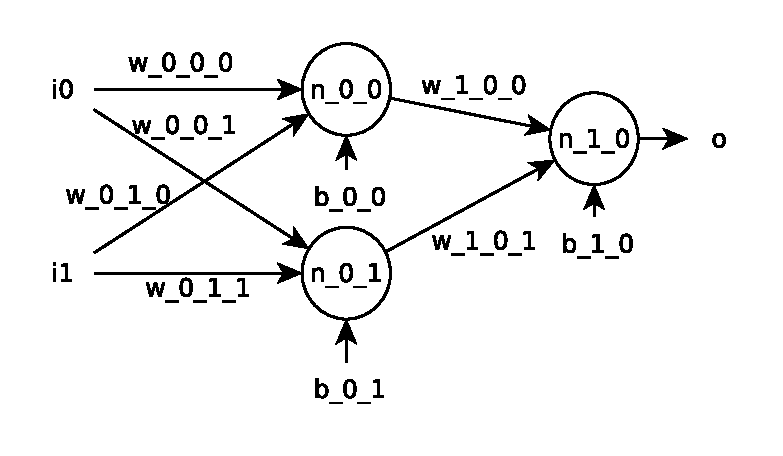
\includegraphics[width=0.75\textwidth]{Figs/arquitetura.pdf}
	\end{figure}

\end{frame}


% --- SLIDE: Experimento 4 (Arquitetura do Neurônio) ---
\begin{frame}{Experimento 5: Integração e Simulação (ModelSim)}
	\justifying
	A rede neural para a porta AND foi integrada em uma estrutura hierárquica e submetida a dois tipos de validação antes da gravação no FPGA:
	
	\begin{itemize}
		\item \textbf{Simulação Comportamental:} Validou-se a funcionalidade matemática. A FSM percorreu todos os estados e gerou os valores de saída esperados conforme o treinamento em PyTorch.
		\item \textbf{Simulação de Timing (Gate-Level):} Utilizou-se a \textit{Netlist} gerada pelo Quartus para o chip da DE0-Nano. 
		\begin{itemize}
			\item \textbf{Resultado:} Confirmou-se que as operações de ponto flutuante estabilizam dentro do período de clock de 50MHz, sem violações de \textit{setup} ou \textit{hold}.
		\end{itemize}
		\item \textbf{Verificação:} O sinal \texttt{Ready} comportou-se de forma estável, permitindo a leitura correta do resultado final após $\approx X$ ciclos de clock.
	\end{itemize}
\end{frame}






% --- SLIDE: Experimento 5 (Implementação e Resultados) ---
\begin{frame}{Experimento 5: Mapeamento Físico e Hardware}
	\justifying
	Para a implementação na placa DE0-Nano, foi desenvolvido um componente \textbf{Top Wrapper} para converter sinais digitais simples em dados de ponto flutuante:
	
	\begin{itemize}
		\item \textbf{Entradas (Switches):} As chaves físicas (SW0 e SW1) foram mapeadas para injetar constantes IEEE-754 ($0.0$ ou $1.0$) na rede.
		\item \textbf{Controle (Push-Button):} Um botão físico foi configurado para disparar o sinal \texttt{Start}, iniciando o processamento da FSM.
		\item \textbf{Saída (LEDs):} 
		\begin{itemize}
			\item Um comparador de magnitude foi implementado para acender o LED apenas se a saída da rede for $> 0.5$.
			\item Um segundo LED foi utilizado para sinalizar o estado \texttt{Ready}.
		\end{itemize}
	\end{itemize}
\end{frame}



\begin{frame}{Experimento 5: Validação da Porta AND}
	\justifying
	A tabela abaixo apresenta os resultados obtidos após a programação da placa, comparando a saída teórica com os valores extraídos via Signal Tap e LEDs:
	
	\begin{table}
		\centering
		\small
		\begin{tabular}{|c|c|c|c|c|}
			\hline
			\textbf{A} & \textbf{B} & \textbf{Teoria (AND)} & \textbf{Saída FP (Rede)} & \textbf{LED Status} \\ \hline
			0 & 0 & 0 & 0.0000... & APAGADO \\ \hline
			0 & 1 & 0 & 0.0001... & APAGADO \\ \hline
			1 & 0 & 0 & 0.0001... & APAGADO \\ \hline
			1 & 1 & 1 & 0.9998... & ACESO \\ \hline
		\end{tabular}
	\end{table}
	
	\begin{block}{Conclusão}
		A rede neural convergiu com precisão elevada. A pequena variação decimal ($0.9998$ em vez de $1.0$) é característica da função de ativação Sigmóide, sendo interpretada corretamente pelo hardware.
	\end{block}
\end{frame}



\begin{frame}{Experimento 5: Relatório de Síntese}
	\justifying
	A imagem abaixo detalha a ocupação da área lógica na Cyclone IV após a síntese final do projeto:
	
	\begin{figure}
		\centering
		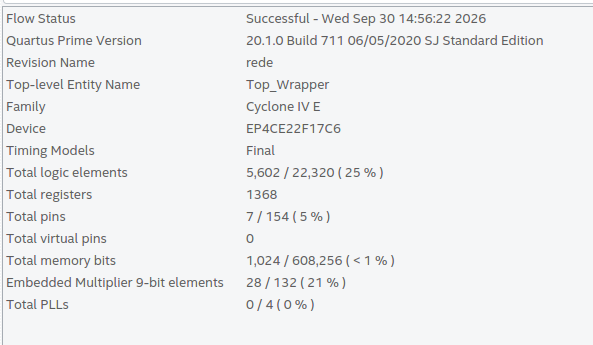
\includegraphics[width=0.45\textwidth]{Figs/fig12.png}
	\end{figure}
	
	\begin{itemize}
		\item \textbf{Eficiência:} O uso de blocos de DSP dedicados permitiu a implementação de multiplicadores de ponto flutuante sem sobrecarregar as LUTs (Logic Elements).
		\item \textbf{Escalabilidade:} O baixo consumo de recursos indica que a DE0-Nano suportaria redes significativamente maiores com a mesma arquitetura modular.
	\end{itemize}
\end{frame}





\begin{frame}[allowframebreaks]{Referências Bibliográficas}
	\footnotesize % Diminui o tamanho da fonte para caber melhor
	
	\begin{itemize}
		\item SAMPAIO, Renato. \textbf{Arquiteturas de hardware para aceleração de algoritmos de controle preditivo não-linear}. 2018. 120 f. Tese (Doutorado em Engenharia Mecânica) — Universidade de Brasília, Brasília, 2018.
		
		\vspace{0.4cm}
		
		\item TRIANA, Mario Andrés Pastrana. \textbf{Controle baseado em comportamento aplicado à robótica móvel usando hardware reconfigurável}. Orientador: Daniel Mauricio Muñoz Arboleda. 2022. 88 f. Dissertação (Mestrado em Sistemas Mecatrônicos) — Universidade de Brasília, Brasília, 2022.
		
		\vspace{0.4cm}
		
		\item GONÇALVES, André Ricardo. \textbf{Redes Neurais Artificiais}. Departamento de Engenharia de Computação e Automação Industrial (DCA) — UNICAMP, Campinas, SP.
		
		
		\item SILVA, Ivan Nunes da; SPATTI, Danilo Hernane; FLAUZINO, Rogério Andrade. Redes neurais artificiais para engenharia e ciências aplicadas: curso prático. São Paulo: Artliber Editora, 2010. 399 p.
		
		
	\end{itemize}
\end{frame}









\end{document}
